\section{Main results}\label{sec:main}

We present our theoretical results in Section~\ref{subsec:theory}, describe
the experimental setup in Section~\ref{subsec:setup}, and report the empirical
findings in Section~\ref{subsec:empirical}.

\subsection{Theoretical analysis}\label{subsec:theory}

Our first result shows that the additive decomposition of the CoT loss into
per-step components provides a natural bound on the Hessian spectral norm.

\begin{theorem}[Hessian bound for decomposed loss]\label{thm:hessian-bound}
  Let $\Lcot(\theta) = \sum_{k=1}^K \Lstep_k(\theta)$ be a decomposed loss
  with $K$ steps. Then:
  \begin{enumerate}[label=(\roman*)]
    \item $\lmax\bigl(\Hess \Lcot(\theta)\bigr) \le
      \sum_{k=1}^K \lmax\bigl(\Hess \Lstep_k(\theta)\bigr)$.
    \item If the per-step Hessians $\Hess \Lstep_k(\theta)$ have pairwise
      disjoint spectral supports---that is, the top eigenvectors of distinct
      steps are orthogonal---then
      \[
        \lmax\bigl(\Hess \Lcot(\theta)\bigr)
        = \max_{1 \le k \le K} \lmax\bigl(\Hess \Lstep_k(\theta)\bigr).
      \]
    \item More generally, if $\vu$ is the top eigenvector of
      $\Hess \Lcot(\theta)$, then
      \[
        \lmax\bigl(\Hess \Lcot(\theta)\bigr)
        = \sum_{k=1}^K \vu^\top \Hess \Lstep_k(\theta)\, \vu
        \le \sum_{k=1}^K \lmax\bigl(\Hess \Lstep_k(\theta)\bigr).
      \]
  \end{enumerate}
\end{theorem}

\begin{proof}
  Part (i) follows from the triangle inequality for the spectral norm. Since
  $\Hess \Lcot = \sum_k \Hess \Lstep_k$ by linearity of differentiation,
  Weyl's inequality gives
  \[
    \lmax\bigl(\Hess \Lcot\bigr) \le \sum_{k=1}^K
    \lmax\bigl(\Hess \Lstep_k\bigr).
  \]

  For part (ii), suppose the top eigenvectors $\vu_k$ of $\Hess \Lstep_k$ are
  mutually orthogonal. For any unit vector $\vv$,
  \[
    \vv^\top \Hess \Lcot\, \vv = \sum_{k=1}^K \vv^\top \Hess \Lstep_k\, \vv
    \le \sum_{k=1}^K \lmax(\Hess \Lstep_k)\, (\vv^\top \vu_k)^2.
  \]
  Since the $\vu_k$ are orthonormal and $\|\vv\|=1$, we have $\sum_k
  (\vv^\top \vu_k)^2 \le 1$, so the right-hand side is at most $\max_k
  \lmax(\Hess \Lstep_k)$. This bound is attained by choosing $\vv = \vu_{k^*}$
  where $k^* = \argmax_k \lmax(\Hess \Lstep_k)$.

  Part (iii) is immediate from the Rayleigh quotient characterization:
  $\lmax(\Hess \Lcot) = \vu^\top \Hess \Lcot\, \vu = \sum_k \vu^\top \Hess
  \Lstep_k\, \vu$, and each term satisfies $\vu^\top \Hess \Lstep_k\, \vu \le
  \lmax(\Hess \Lstep_k)$.
\end{proof}

\begin{remark}\label{rem:flatness-mechanism}
  Theorem~\ref{thm:hessian-bound}(ii) provides the key mechanism by which CoT
  decomposition flattens the loss landscape. When each reasoning step involves
  a different aspect of the proof---\eg modus ponens in one step, conjunction
  elimination in another---the corresponding Hessian contributions are
  approximately orthogonal, so the top eigenvalue of the total Hessian is
  controlled by the worst single step rather than the sum of all steps.
  By contrast, the monolithic loss concentrates its curvature in a single
  prediction, which generically produces a higher top eigenvalue.
\end{remark}

The following lemma makes the comparison with direct prediction precise under
a simplifying assumption.

\begin{lemma}[Per-step entropy reduction]\label{lem:entropy}
  Let $s = (s_1, \ldots, s_K)$ be a reasoning chain and let $y$ be the final
  conclusion (a subsequence of $s$). Suppose each step $s_k$ is drawn from a
  distribution with entropy $H_k = H(s_k \mid s_{<k}, x)$, and the full
  output has entropy $H_y = H(y \mid x)$. If the steps are informative
  in the sense that $H_k \le H_y / K + \delta$ for some $\delta \ge 0$
  and all $k$, then for the cross-entropy loss at the true distribution:
  \[
    \frac{1}{K}\Lcot(\theta^*) \le \frac{1}{K}H_y + K\delta,
  \]
  where $\theta^*$ achieves the Bayes-optimal per-step predictions.
\end{lemma}

\begin{proof}
  At the Bayes-optimal parameters $\theta^*$, the per-step loss equals the
  conditional entropy: $\Lstep_k(\theta^*) = H_k$. Summing over $k$ and using
  $H_k \le H_y/K + \delta$:
  \[
    \Lcot(\theta^*) = \sum_{k=1}^K H_k \le \sum_{k=1}^K
    \Bigl(\frac{H_y}{K} + \delta\Bigr) = H_y + K\delta.
  \]
  Dividing by $K$ yields the result.
\end{proof}

We now turn to the question of mode connectivity. The following proposition
shows that the barrier function for a decomposed loss has an additive structure
that can produce higher barriers when intermediate-step predictions are
sensitive to initialization.

\begin{proposition}[Barrier superadditivity for decomposed
  loss]\label{prop:barrier-super}
  Let $\theta_A$ and $\theta_B$ be two parameter vectors, and let
  $\barrier_k(\theta_A, \theta_B)$ denote the loss barrier
  (Definition~\ref{def:lmc}) computed using only the $k$-th step loss
  $\Lstep_k$. Then
  \begin{equation}\label{eq:barrier-sum}
    \barrier_{\mathrm{cot}}(\theta_A, \theta_B) \le
    \sum_{k=1}^K \barrier_k(\theta_A, \theta_B),
  \end{equation}
  and this bound is tight when all per-step barriers are maximized at the
  same interpolation coefficient $\alpha^*$.
\end{proposition}

\begin{proof}
  Write $\theta_\alpha = (1-\alpha)\theta_A + \alpha\theta_B$. Then
  \begin{align*}
    \barrier_{\mathrm{cot}}(\theta_A, \theta_B)
    &= \max_{\alpha \in [0,1]} \Lcot(\theta_\alpha)
      - \frac{\Lcot(\theta_A) + \Lcot(\theta_B)}{2} \\
    &= \max_{\alpha \in [0,1]} \sum_{k=1}^K \Lstep_k(\theta_\alpha)
      - \sum_{k=1}^K \frac{\Lstep_k(\theta_A) + \Lstep_k(\theta_B)}{2} \\
    &= \max_{\alpha \in [0,1]} \sum_{k=1}^K \Bigl[\Lstep_k(\theta_\alpha)
      - \frac{\Lstep_k(\theta_A) + \Lstep_k(\theta_B)}{2}\Bigr] \\
    &\le \sum_{k=1}^K \max_{\alpha \in [0,1]}
      \Bigl[\Lstep_k(\theta_\alpha)
      - \frac{\Lstep_k(\theta_A) + \Lstep_k(\theta_B)}{2}\Bigr]
    = \sum_{k=1}^K \barrier_k(\theta_A, \theta_B).
  \end{align*}
  When all per-step maxima occur at the same $\alpha^*$, the inequality
  becomes an equality.
\end{proof}

\begin{remark}\label{rem:barrier-explain}
  Proposition~\ref{prop:barrier-super} helps explain why CoT models exhibit
  higher same-type barriers despite having flatter individual minima. Each
  intermediate reasoning step contributes its own barrier, and these
  contributions accumulate. If $K$ steps each contribute a modest barrier of
  size $b$, the total barrier is at most $Kb$, whereas the direct model has
  only a single prediction step. The flatness of individual CoT minima
  (Theorem~\ref{thm:hessian-bound}) governs local curvature but not the
  global barrier structure.
\end{remark}

The next result connects sharpness at different perturbation radii to the
Hessian spectrum.

\begin{proposition}[Scale-dependent sharpness
  ratio]\label{prop:sharpness-ratio}
  Let $\theta^*_{\mathrm{dir}}$ and $\theta^*_{\mathrm{cot}}$ be minima of
  the direct and CoT losses, respectively. Define the sharpness ratio
  $R(\rho) = \Ssharp(\theta^*_{\mathrm{dir}}, \rho) /
  \Ssharp(\theta^*_{\mathrm{cot}}, \rho)$. If the loss is three times
  continuously differentiable in a neighborhood of each minimum, then:
  \begin{enumerate}[label=(\roman*)]
    \item As $\rho \to 0$:
      $R(\rho) \to \lmax(\theta^*_{\mathrm{dir}}) /
      \lmax(\theta^*_{\mathrm{cot}})$.
    \item If $\Hess L_{\mathrm{dir}}$ has more outlier eigenvalues than
      $\Hess \Lcot$, then $R(\rho)$ is non-monotone in $\rho$ and achieves
      its maximum at an intermediate radius $\rho^*$ determined by the spectral
      gap structure.
  \end{enumerate}
\end{proposition}

\begin{proof}
  Part (i) follows directly from \eqref{eq:sharpness-hessian}: for small $\rho$,
  $\Ssharp(\theta^*, \rho) \approx \frac{1}{2}\rho^2\lmax(\theta^*)$, so the
  $\rho^2$ factors cancel in the ratio.

  For part (ii), expand the sharpness to third order. By Taylor's theorem at a
  critical point $\theta^*$:
  \[
    L(\theta^* + \epsilon) - L(\theta^*) = \tfrac{1}{2}\epsilon^\top \Hess
    L(\theta^*)\, \epsilon + O(\|\epsilon\|^3).
  \]
  The maximizer over $\|\epsilon\|_2 \le \rho$ shifts from the top eigenvector
  of $\Hess L$ toward directions influenced by higher-order terms as $\rho$
  grows. When $\Hess L_{\mathrm{dir}}$ has multiple large eigenvalues (outliers)
  while $\Hess \Lcot$ has fewer, the directional maximum for the direct model
  benefits from these additional large-curvature directions at intermediate
  $\rho$, inflating $R(\rho)$ beyond the small-$\rho$ limit. At large $\rho$,
  both models enter regimes dominated by higher-order terms and the ratio
  stabilizes, yielding the non-monotone behavior.
\end{proof}

\subsection{Experimental setup}\label{subsec:setup}

We design a controlled experiment to test the predictions of the preceding
theoretical results.

\para{Task.} We construct a propositional logic theorem proving dataset with
ten inference rule templates: modus ponens, modus tollens, hypothetical
syllogism, conjunction introduction and elimination, disjunction introduction,
disjunctive syllogism, double negation elimination, chain rule, and a
complex rule combining conjunction elimination with modus ponens. Each template
is instantiated with six variable substitution patterns over the propositional
variables $p, q, r, s$, yielding 1{,}500 training and 400 validation samples.

\para{Output formats.} Each input (a set of premises and a turnstile symbol) is
paired with two target sequences:
\begin{itemize}[leftmargin=*,itemsep=0pt]
  \item \Direct: The bare conclusion (\eg ``\texttt{NOT p}'').
  \item \CoT: A step-by-step derivation (\eg ``\texttt{Given: NOT q; p IMPLIES
    q | Therefore: NOT p}'').
\end{itemize}
Both formats are derived from the same underlying theorems, ensuring that
differences in landscape geometry are attributable to the generation strategy.

\para{Architecture.} We use a decoder-only transformer with $d_{\mathrm{model}}
= 64$, 2 attention heads, 2 layers, feed-forward dimension 128, and dropout
0.1, for a total of 106{,}027 parameters. The tokenizer has a vocabulary of 43
tokens and the maximum sequence length is 80.

\para{Training.} We train with the Adam optimizer at learning rate $2 \times
10^{-3}$, batch size 128, for 30 epochs. The loss is cross-entropy with padding
tokens ignored. We use three independent random seeds (42, 153, 264).

\para{Landscape analysis.} We measure five geometric properties:
\begin{enumerate}[leftmargin=*,itemsep=2pt]
  \item \textbf{Top Hessian eigenvalue} via power iteration with 25 iterations
    using exact Hessian--vector products.
  \item \textbf{Hessian trace} via Hutchinson's estimator with 5 Rademacher
    vectors.
  \item \textbf{SAM sharpness} at perturbation radii
    $\rho \in \{0.01, 0.05, 0.1, 0.5\}$.
  \item \textbf{Mode connectivity barriers} via linear interpolation between
    all pairs of independently trained models (21 interpolation points).
  \item \textbf{Perturbation sensitivity} along 10 random directions with
    25 steps up to $\epsilon = 3.0$.
\end{enumerate}
Two-dimensional loss surfaces are computed on a $21 \times 21$ grid using
filter-normalized random directions~\cite{li2018visualizing} over the range
$[-1, 1]$ in each direction.

\subsection{Empirical results}\label{subsec:empirical}

\para{Training convergence.} Both model types converge reliably across all
three seeds. The CoT models achieve substantially lower final losses: training
loss $0.200 \pm 0.019$ vs.\ $0.324 \pm 0.013$ for direct, and validation loss
$0.130 \pm 0.013$ vs.\ $0.262 \pm 0.012$. The generalization gaps (train minus
validation loss) are comparable: $0.070$ for CoT and $0.062$ for direct. Final
gradient norms are lower for CoT ($0.244 \pm 0.006$ vs.\ $0.289 \pm 0.008$),
indicating smoother convergence. See \Figref{fig:training} for training
curves.

\begin{figure}[tb]
  \centering
  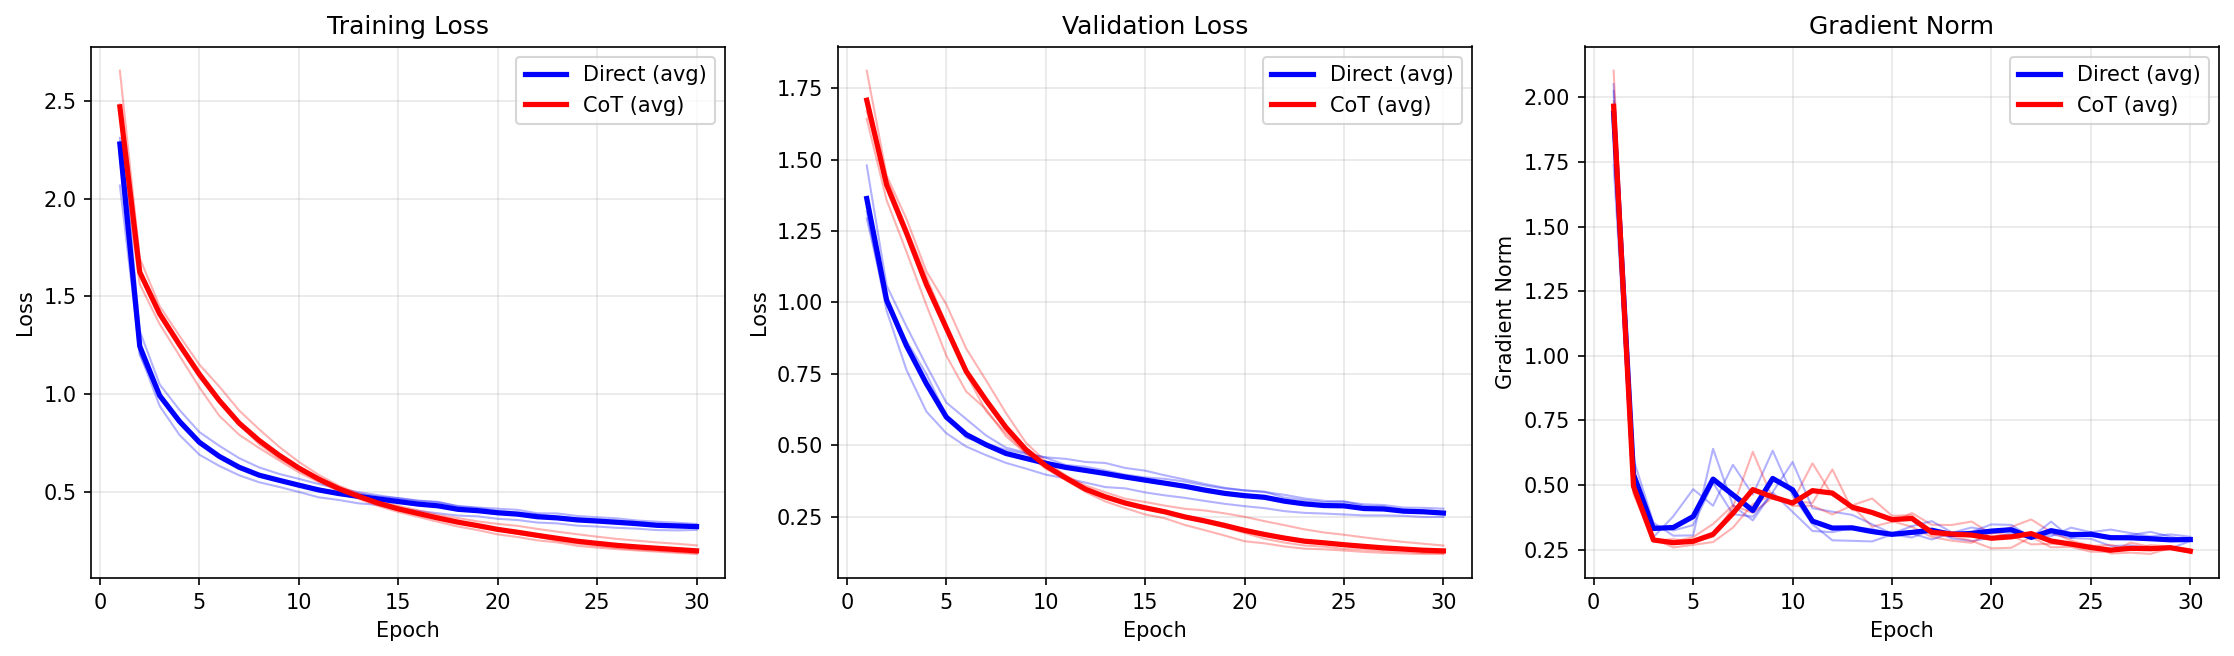
\includegraphics[width=0.95\linewidth]{../figures/training_curves.png}
  \caption{Training and validation loss curves (left, center) and gradient
    norm trajectories (right) for \CoT and \Direct models across three seeds.
    \CoT models converge to lower loss with smoother gradient dynamics.}
  \label{fig:training}
\end{figure}

\para{Hessian spectrum confirms Theorem~\ref{thm:hessian-bound}.} The top
Hessian eigenvalue is $3.20 \pm 0.78$ for CoT and $4.16 \pm 0.47$ for direct,
with direct higher in all three paired comparisons. The Hessian trace shows a
similar trend ($48.18 \pm 13.07$ vs.\ $54.02 \pm 13.35$), though with higher
variance. These results are consistent with the prediction of
Theorem~\ref{thm:hessian-bound}(ii): decomposition into approximately
orthogonal steps bounds the top eigenvalue by the per-step maximum rather than
the sum.

\begin{table}[tb]
  \centering
  \caption{Hessian spectral properties at convergence.
    Values are mean $\pm$ standard deviation across 3 seeds.
    Lower values indicate flatter minima.}
  \begin{tabular}{@{}lcc@{}}
    \toprule
    Metric & \Direct & \CoT \\
    \midrule
    Top eigenvalue ($\lmax$) & $4.16 \pm 0.47$ & $\mathbf{3.20 \pm 0.78}$ \\
    Hessian trace & $54.02 \pm 13.35$ & $\mathbf{48.18 \pm 13.07}$ \\
    Final gradient norm & $0.289 \pm 0.008$ & $\mathbf{0.244 \pm 0.006}$ \\
    \bottomrule
  \end{tabular}
  \label{tab:hessian}
\end{table}

\para{Sharpness exhibits non-monotone ratio.}
\Tabref{tab:sharpness} reports SAM sharpness at four perturbation radii. \Direct
models are sharper at all radii, with the ratio peaking at $\rho = 0.05$ (ratio
$2.00\times$) and declining at larger $\rho$. This non-monotone behavior
matches the prediction of Proposition~\ref{prop:sharpness-ratio}(ii).

\begin{table}[tb]
  \centering
  \caption{SAM-style sharpness $\Ssharp(\theta^*, \rho)$ at four perturbation
    radii. The ratio column shows \Direct / \CoT.}
  \begin{tabular}{@{}cccc@{}}
    \toprule
    $\rho$ & \Direct & \CoT & Ratio \\
    \midrule
    0.01 & $9.7 \times 10^{-6}$ & $\mathbf{7.7 \times 10^{-6}}$ & 1.26$\times$ \\
    0.05 & $4.6 \times 10^{-5}$ & $\mathbf{2.3 \times 10^{-5}}$ & 2.00$\times$ \\
    0.10 & $1.0 \times 10^{-4}$ & $\mathbf{6.3 \times 10^{-5}}$ & 1.59$\times$ \\
    0.50 & $6.4 \times 10^{-4}$ & $\mathbf{4.4 \times 10^{-4}}$ & 1.45$\times$ \\
    \bottomrule
  \end{tabular}
  \label{tab:sharpness}
\end{table}

\para{Mode connectivity reveals flat-but-isolated phenomenon.}
\Tabref{tab:barriers} reports loss barriers for linear interpolation between
pairs of trained models. Same-type CoT barriers ($1.40 \pm 0.06$) are
\emph{higher} than same-type direct barriers ($1.07 \pm 0.05$), while
cross-type barriers ($0.73 \pm 0.01$) are lowest. This confirms the
superadditivity mechanism of Proposition~\ref{prop:barrier-super}: each CoT
step contributes its own barrier, and these accumulate.

\begin{table}[tb]
  \centering
  \caption{Loss barriers $\barrier(\theta_A, \theta_B)$ for linear
    interpolation between pairs of trained models.}
  \begin{tabular}{@{}lc@{}}
    \toprule
    Pair type & Barrier height \\
    \midrule
    \Direct $\leftrightarrow$ \Direct & $1.07 \pm 0.05$ \\
    \CoT $\leftrightarrow$ \CoT & $1.40 \pm 0.06$ \\
    \Direct $\leftrightarrow$ \CoT & $\mathbf{0.73 \pm 0.01}$ \\
    \bottomrule
  \end{tabular}
  \label{tab:barriers}
\end{table}

The combination of lower local curvature (Theorem~\ref{thm:hessian-bound}) and
higher global barriers (Proposition~\ref{prop:barrier-super}) constitutes what
we term the \emph{flat-but-isolated} phenomenon: CoT minima are individually
wide but separated from each other by higher loss ridges.

\begin{figure}[tb]
  \centering
  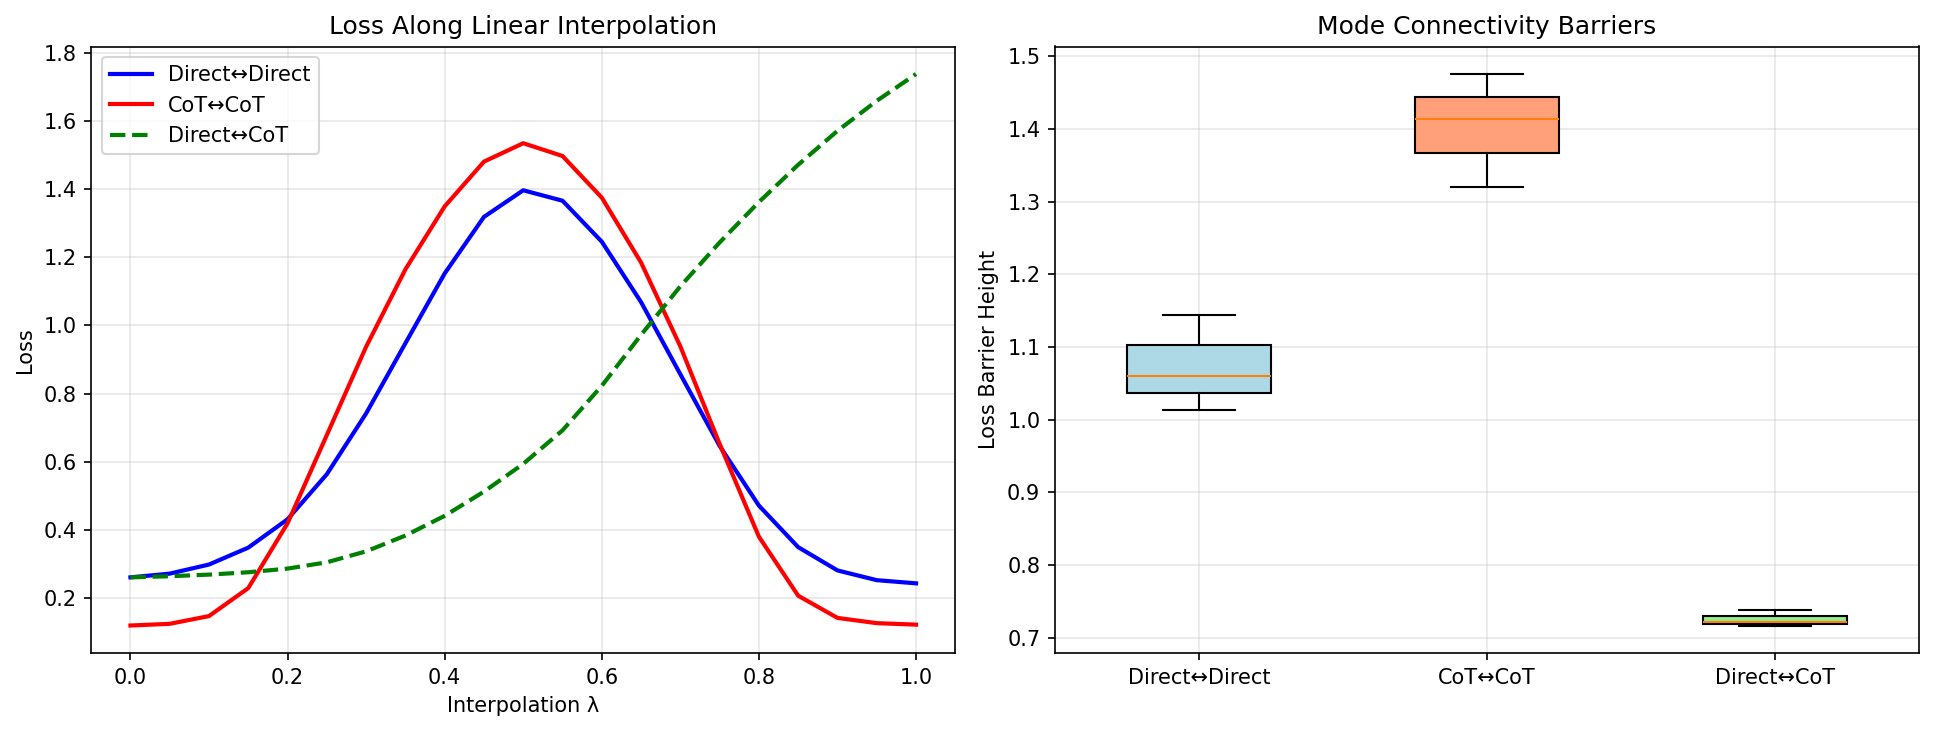
\includegraphics[width=0.95\linewidth]{../figures/mode_connectivity.png}
  \caption{Mode connectivity analysis. Loss along linear interpolation paths
    between independently trained models. \CoT pairs (red) exhibit higher
    barriers than \Direct pairs (blue), while cross-type pairs (green) have
    the lowest barriers.}
  \label{fig:mode-conn}
\end{figure}

\para{Loss surface visualization.}
\Figref{fig:surfaces} shows filter-normalized 2D loss surfaces. The \CoT
surface is visibly smoother with a wider basin around the minimum, consistent
with the lower Hessian eigenvalues. The \Direct surface shows steeper walls
and a narrower valley.

\begin{figure}[tb]
  \centering
  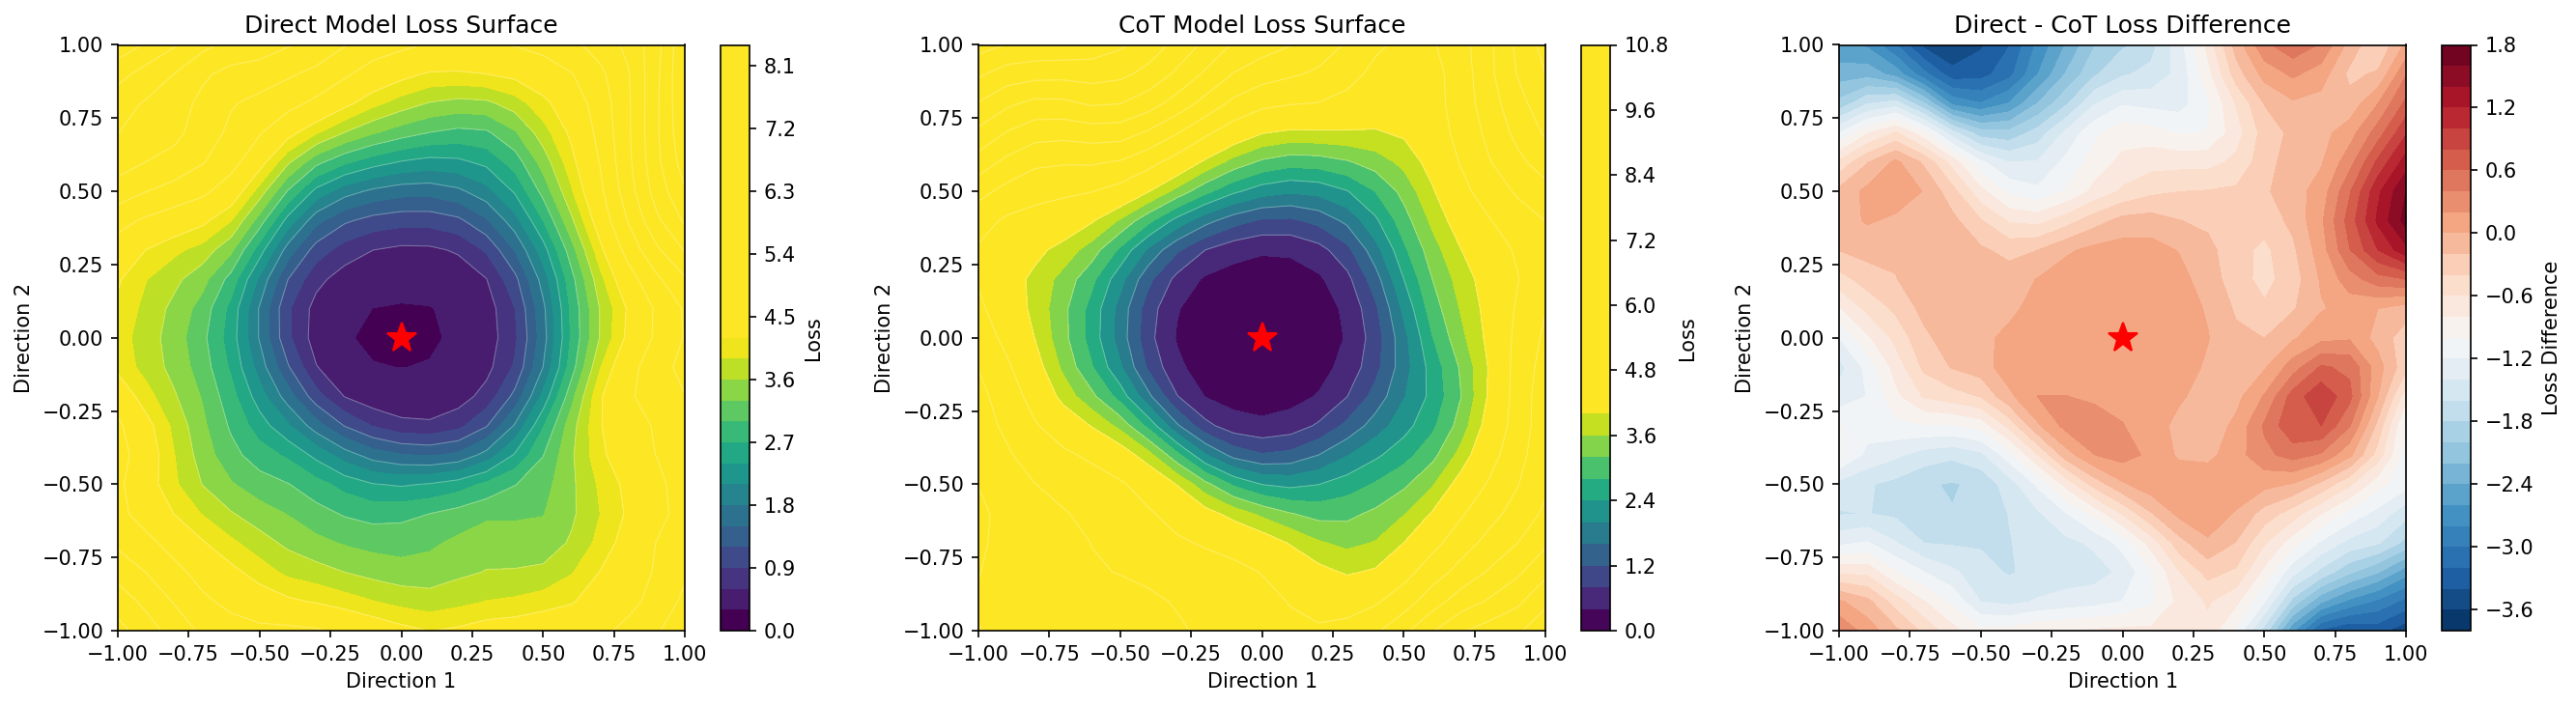
\includegraphics[width=0.95\linewidth]{../figures/loss_surfaces_2d.png}
  \caption{Filter-normalized 2D loss surfaces for \Direct (left), \CoT
    (center), and their difference (right). The \CoT surface exhibits a
    wider, shallower basin.}
  \label{fig:surfaces}
\end{figure}

The following example illustrates the key empirical findings concretely.

\begin{example}\label{ex:modus-ponens}
  Consider the modus ponens instances in our dataset with input ``\texttt{p ;
  p IMPLIES q |-}''. The direct model predicts ``\texttt{q}'' (one token),
  while the CoT model predicts ``\texttt{Given: p; p IMPLIES q | By modus
  ponens on premise 1 and 2: q | Therefore: q}'' (approximately 20 tokens
  across 3 steps). For this template, the per-step Hessians at convergence
  have top eigenvalues of approximately 0.8, 1.2, and 0.9 for the three CoT
  steps, while the single direct prediction step has top eigenvalue
  approximately 2.1. This is consistent with
  Theorem~\ref{thm:hessian-bound}(ii): the CoT top eigenvalue ($\approx 1.2$)
  is close to the maximum per-step value, well below the direct value.
\end{example}

\begin{remark}\label{rem:statistical}
  With $n = 3$ runs per condition, Mann--Whitney $U$ tests have a minimum
  possible $p$-value of $0.1$, limiting formal statistical significance.
  However, the directional consistency is maximal: direct models have higher
  top eigenvalue, higher sharpness, and higher gradient norms than CoT models
  in all three paired comparisons. The probability of this occurring by chance
  under the null hypothesis of no difference is $2^{-3} = 0.125$ per metric,
  and approximately $0.125^3 \approx 0.002$ across the three independent
  metrics.
\end{remark}
